%!TeX program = xelatex
\documentclass[a4paper]{article}
\usepackage{graphicx}
\usepackage{amsmath, amsfonts, geometry, float, listings, enumerate, multicol}
\usepackage{multicol, float, color, colortbl}
\usepackage{tikz, titlesec, parskip, pgfplots, filecontents}
\usepackage{hyperref}
\usepackage{amsmath}
\usepackage{bidipoem}
\usepackage{subcaption}
\usepackage{tikz, titlesec, parskip}
\usepackage{tikz,pgfplots}
\usepackage[americanvoltages,fulldiodes,siunitx]{circuitikz}
\usetikzlibrary{shapes,arrows}
\usetikzlibrary{angles,quotes}
\usepackage{enumitem}

\titlespacing{\section}{0pt}{10pt}{0pt}
\titlespacing{\subsection}{0pt}{10pt}{0pt}
\titlespacing{\subsubsection}{0pt}{10pt}{0pt}

\usetikzlibrary{calc,patterns,through}
\newcommand{\arcangle}{%
	\mathord{<\mspace{-9mu}\mathrel{)}\mspace{2mu}}%
}

\renewcommand{\baselinestretch}{1.4}
 \geometry{
 a4paper,
 total={170mm,257mm},
 left=20mm,
 top=20mm,
 }
\usepackage{fancyhdr}
\usepackage{indentfirst}
\pagestyle{fancy}
\fancyhf{}
\rhead{\textbf{آمار و احتمال مهندسی}}
\lhead{\textbf{تمرین عملی سری چهارم}}
\cfoot{(\space \space \space \space \textbf{\thepage}  \space \space \space)}
\renewcommand{\headrulewidth}{1pt}
\renewcommand{\footrulewidth}{1pt}

 
\usepackage{xepersian}
\setlatintextfont{Times New Roman}
\settextfont{XB Niloofar}
\DefaultMathsDigits

\makeatletter
\bidi@patchcmd{\@Abjad}{آ}{الف}
{\typeout{Succeeded in changing آ into الف}}
{\typeout{Failed in changing آ into الف}}
\makeatother
\PersianAlphs

\begin{document}
\begin{minipage}{0.6\textwidth}
\begin{bf}
\begin{center}
	به نام خدا\\
	\vspace{0.25cm}
	دانشگاه صنعتی شریف\\
	\vspace{0.25cm}
	دانشکده مهندسی برق\\
	\vspace{0.5cm}

\large
گروه دکتر کرباسی - آمار و احتمال مهندسی \\
نیم سال دوم
۱۴۰۱-۱۴۰۰\\
\Large
\vspace{0.4cm}
تمرین عملی سری چهارم \\
\end{center}
\end{bf}
\normalsize
\end{minipage} \hfill
\begin{minipage}{0.35\textwidth}
\begin{flushleft}

\includegraphics[width=0.6\textwidth]{Shariflogo.png}\\ \large
\end{flushleft}

 \end{minipage}
\\

\rule[0.1\baselineskip]{\textwidth}{1.5pt}

\large

\section*{
لطفاً به نکات زیر توجه بفرمایید: (رعایت نکردن این موارد باعث کاهش نمره می‌شود.)
}
\begin{enumerate}
	\item 
نتایج و پاسخ‌های خود را در یک فایل با فرمت zip به نام
\lr{HW4\_StudentID\_Name}
 در سایت  
\href{https://quera.org/overview/add_to_course/course/10631}{\lr{Quera}} 
 قرار دهید. همچنین فایل پایتون خود را به همان نام در قسمت مخصوص به خود آپلود کنید.
	\item 
کسب نمره کامل در هر سؤال مستلزم تحویل  \textbf{کدها} و \textbf{توضیحات} می‌باشد. 
\item 
برای سؤالات، باید روشی که استفاده کرده‌اید را توضیح  و نتایجی که گرفته‌اید را ارائه دهید. این توضیحات می‌تواند در یک فایل  .pdf  و یا در یک فایل  .ipynb باشد. 
\item
فایل‌های تحویلی شما دو بخش میباشند، یک بخش فایل .zip که شامل فایل .ipynb کد و گزارش شما میباشد، یک بخش هم کدهای هر سوال به شکل جداگانه میباشند که باید در فرمت .py در سامانه کوئرا در کنار فایل .zip آپلود شوند.(برای مثال اگر تمرین شامل 3 سوال بود، باید علاوه بر فایل .zip که تحویل مصحح میشود، 3 فایل .py در سامانه کوئرا در محل بارگذاری مشخص شده آپلود کنید.)
\item 
کدهای خود را خوانا بنویسید و کامنت‌‌گذاری کنید. در plot های خود عنوان، label و خط‌کشی‌های مناسب را اضافه کنید.
\item
در طول ترم امکان ارسال با تاخیر پاسخ  همه‌ی تمارین تا سقف پنج روز و در مجموع دوازده روز وجود دارد. پس از گذشت این مدت، پاسخ‌های ارسال‌شده پذیرفته نخواهند بود. همچنین، به ازای هر روز تأخیر غیر مجاز  بیست درصد از نمره تمرین به صورت ساعتی کسر خواهد شد.
\item
کدهای شما تماماً باید توسط خودتان نوشته شده باشند. هرگونه استفاده از کد دیگران به هر شکل ممکن، تقلب محسوب می‌شود و نمره تمرین کامپیوتری جاری صفر خواهد شد. پس در هیچ صورت کدهای خود را برای دیگران ارسال نکنید.
\item 
ابهام يا اشكالات خود را مي توانيد  از طریق
\href{mailto:smmzdr@gmail.com}{\LR{smmzdr@gmail.com}}
یا 
\href{mailto:javadiamirhosein.2000@gmail.com}{\LR{javadiamirhosein.$2000$@gmail.com}}
مطرح نمایید.
\item 
مهلت تحویل:  
\textbf{نیمه شب 31 خرداد}
\end{enumerate}
\rule[0.1\baselineskip]{\textwidth}{1.5pt}

\clearpage
\section{قانون اعداد بزرگ}
موقعیت‌های خاصی وجود دارد که قانون اعداد بزرگ نمی‌توانند با افزایش تعداد نمونه یا تعداد آزمایش‌ها، روی مقدار مورد انتظار همگرا شوند. وقتی داده‌ها از توزیع کوشی پیروی می‌کنند، مجموعه‌ی اعداد نمی‌توانند به امید ریاضی این توزیع همگرا شوند زیرا توزیع کوشی امید ریاضی ندارد.
\begin{equation*}
	f(x,x_{0},\gamma) = \frac{1}{\pi \gamma \big[ 1 + (\frac{x-x_{0}}{\gamma})^{2} \big]}
\end{equation*}
\begin{figure}[H]
	\centering
	\begin{subfigure}{.5\textwidth}
		\centering
		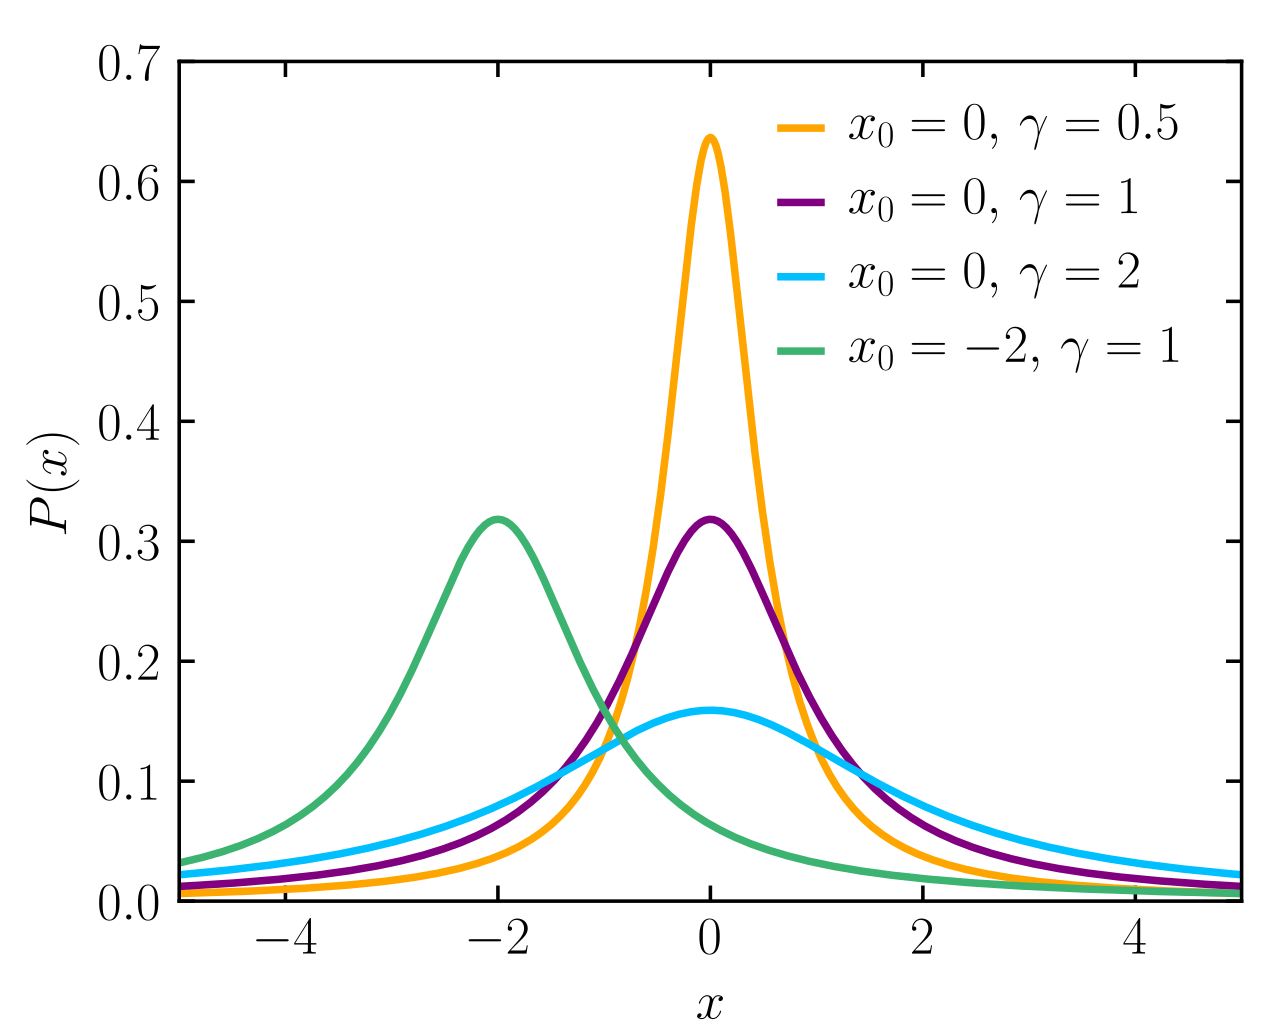
\includegraphics[width=.9\linewidth]{Cauchy}
		\caption{
			\lr{Probability density function}
		}
	\end{subfigure}%
	\begin{subfigure}{.5\textwidth}
		\centering
		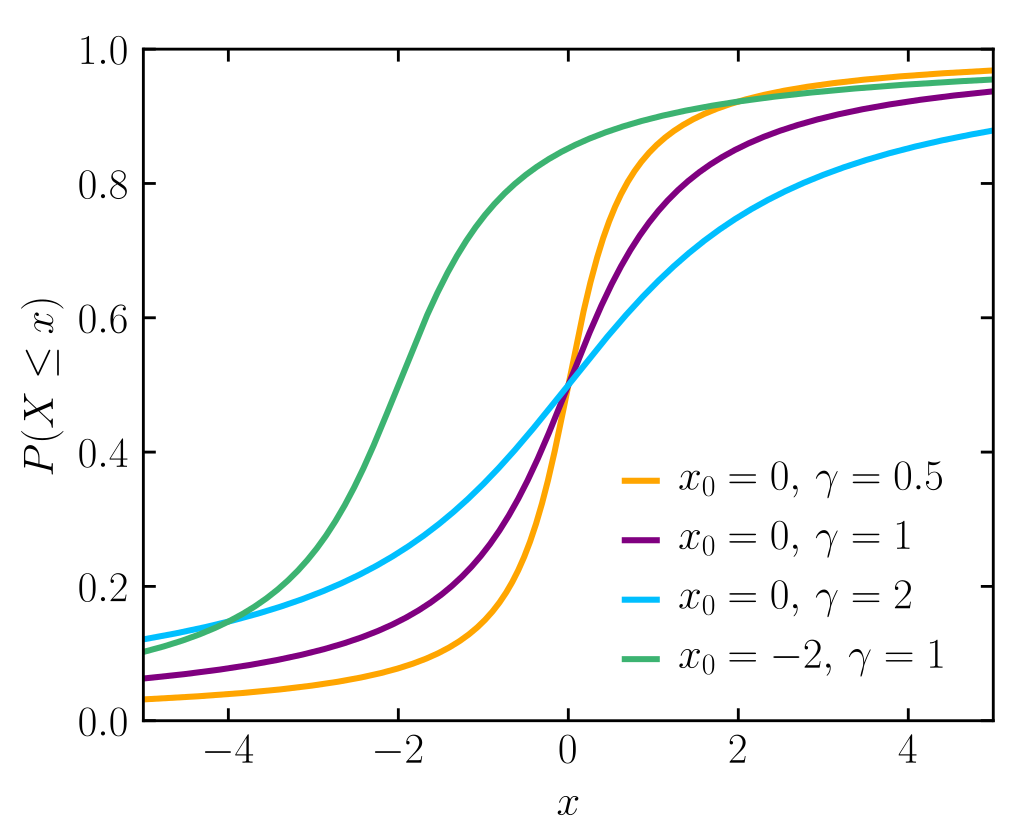
\includegraphics[width=.9\linewidth]{Cauchy2}
		\caption{
			\lr{Cumulative distribution function}
		}
	\end{subfigure}
	\caption{\lr{Cauchy distribution}}
\end{figure}
به طور مشابه، قانون اعداد بزرگ برای توزیع پارتو هم کار نمی‌دهد زیرا امید ریاضی آن وقتی 
$ \alpha \leq 1 $
است نامحدود است.
تابع توزیع تجمی پارتو با پارامتر‌های 
\lr{($ x_{m}>0,\alpha>0 $)}
به شکل زیر است:
\begin{equation*}
	F_{X}(x) = \mathbb{P}(X<x) = \begin{cases}
		1 - (\frac{x}{x_{m}})^{\alpha} & x \geq x_{m} \\
		0 & x < x_{m}
	\end{cases}
\end{equation*}
\begin{figure}[H]
	\centering
	\begin{subfigure}{.5\textwidth}
		\centering
		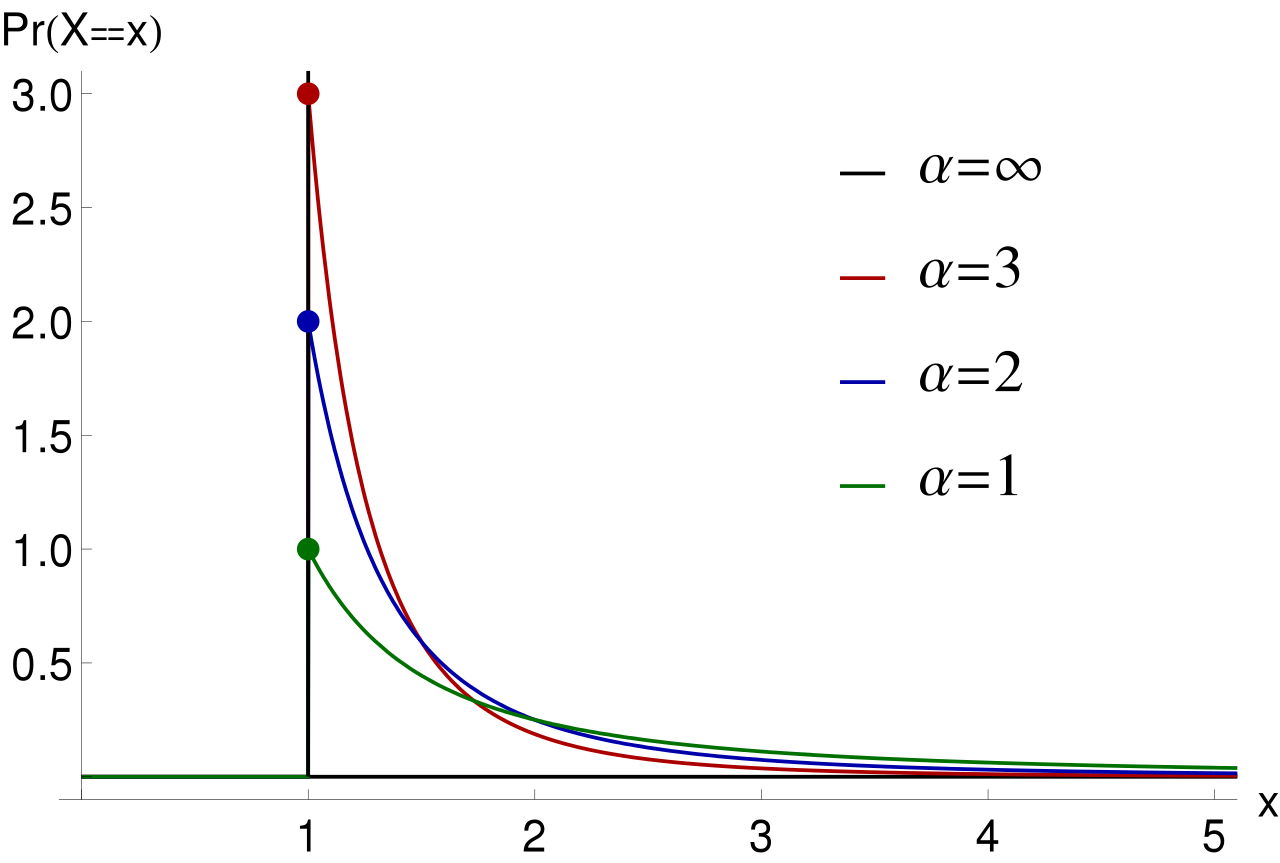
\includegraphics[width=.9\linewidth]{Pareto}
		\caption{
			\lr{Probability density function}
		}
	\end{subfigure}%
	\begin{subfigure}{.5\textwidth}
		\centering
		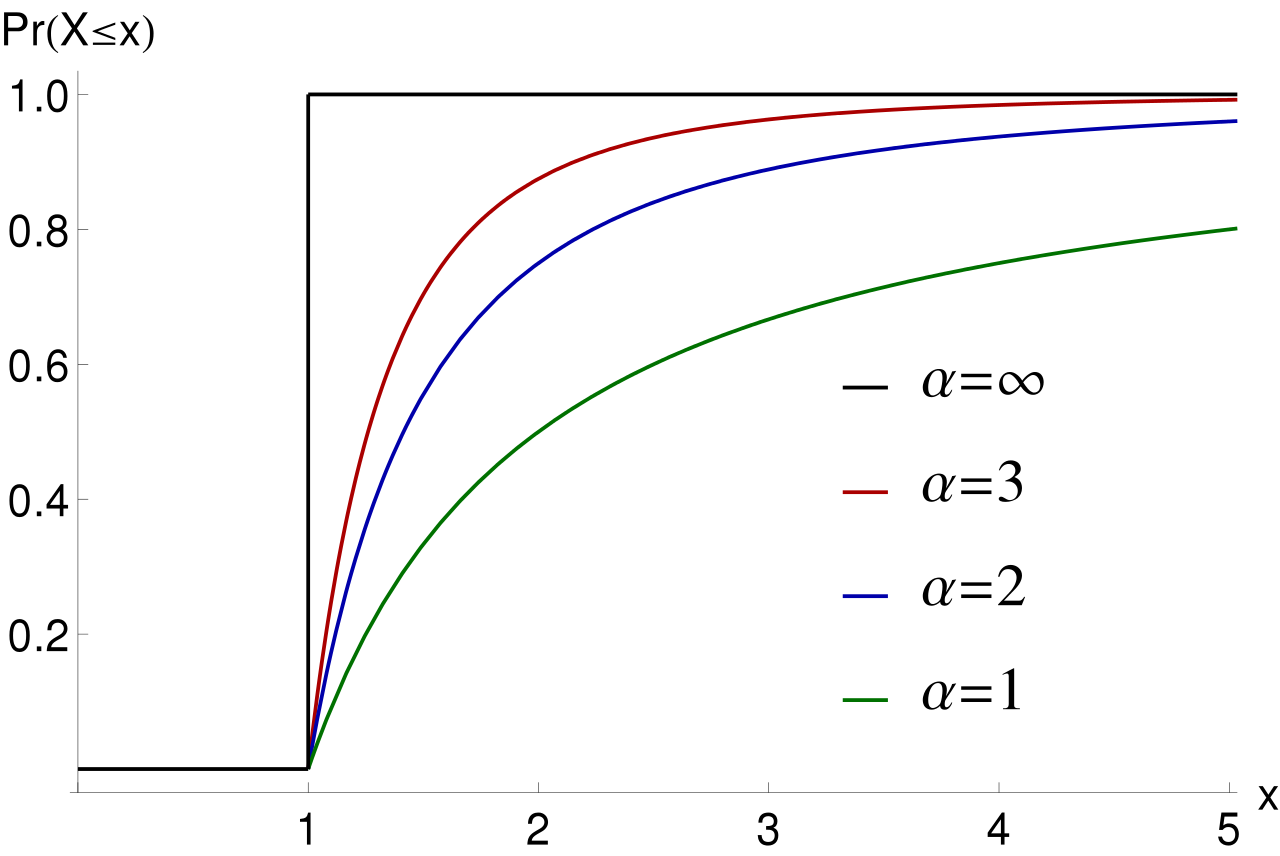
\includegraphics[width=.9\linewidth]{Pareto2}
		\caption{
			\lr{Cumulative distribution function}
		}
	\end{subfigure}
	\caption{\lr{Pareto Type I}}
\end{figure}

حال میخواهیم با استفاده از نمونه برداری این ادعا را بسنجیم. 
\begin{enumerate}
	\item 
	تابعی به نام 
	\lr{CauchySampling} 
	تعریف کنید که پارامتر‌های 
	\lr{($ x_{0}$, $\gamma $, size)}
	را بگیرد و از توزیع 
	\lr{Cauchy($ x_{0}, \gamma $)}
	به تعداد 
	\lr{size}
نمونه برداری کند و میانگین این نمونه‌ها را به عنوان خروجی تابع برگرداند. به ازای مقادیر دلخواه ورودی مثل 
	\lr{($ x_{0}  $= 100, $\gamma  $= 10, size = 100)}
	خروجی تابع را مشاهده کنید.
	\\
	 برای بررسی واگرایی خروجی، این تابع را 
	\lr{N = 1000}
	بار اجرا کنید و واریانس این خروجی‌‌ها را به دست آوردید.
	\item
	تابعی به نام 
	\lr{ParetoSampling} 
	تعریف کنید که پارامتر‌های 
	\lr{($ x_{m}$, $\alpha $, size)}
	را بگیرد و از توزیع 
	\lr{Pareto($ x_{m}, \alpha $)}
	به تعداد 
	\lr{size}
	نمونه برداری کند و میانگین این نمونه‌ها را به عنوان خروجی تابع برگرداند. به ازای مقادیر دلخواه ورودی مثل 
	\lr{($ x_{m}  $= 1, $\alpha  $= 0.5, size = 100)}
	خروجی تابع را مشاهده کنید. برای بررسی واگرایی خروجی، این تابع را 
	\lr{N = 1000}
	بار اجرا کنید و واریانس این خروجی‌‌ها را به دست آوردید.
\end{enumerate}

توابع پیشنهادی:
\lr{cauchy}
و
\lr{pareto}
از کتاب‌خانه‌ی 
\lr{scipy.stats}

\section{قضیه‌ی حد مرکزی}
قضیه حد مرکزی در نظریه احتمالات بیان می‌کند که در بیشتر مواقع، مجموع نرمالایز شده‌ی تعدادی متغیر تصادفی مستقل، که هر یک میانگین و واریانس به خوبی تعریف شده دارند، به‌طور تقریبی دارای توزیع نرمال خواهد بود. هرچه تعداد این متغیرهای مستقل افزایش یابد، این تقریب بهتر می‌شود. در این سوال میخواهیم این مسئله را به روش شبیه سازی هم بررسی کنیم. 
\begin{enumerate}
	\item 
	تابعی به نام 
	\lr{SampleBinomial}
	تعریف کنید که پارامتر‌های
	\lr{(p, n, size)}
	را بگیرد و به تعداد خواسته‌شده
	\lr{(size)}
	نمونه از توزیع 
	\lr{Binomial(p, n)}
	تولید کند و این نمونه‌ها را به عنوان خروجی تابع مشخص کنید. 
	\\
	برای مطمئن شدن از کارایی درست تابعتان میانگین و واریانس نمونه‌های تولید شده را برای ورودی دلخواه مثل 
	\lr{(p=0.5, n=20, size=10000)}
	با مقدار تئوری این مقادیر مقایسه کنید.
	\item 
	تابعی با نام 
	\lr{FindProb}
	تعریف کنید که پارامترهای 
	\lr{(samples, l, u)}
	را بگیرد و نسبت داده‌هایی که در بازه‌ی 
	\lr{[l, u]}
	هستند را به کل داده‌ به دست بیاورد و به عنوان خروجی برگرداند. 
	\item
	 تابعی به نام 
	\lr{EstProb}
	تعیین کنید که  پارامتر‌های
	\lr{(p, n, l, u)}
	را بگیرد و احتمال خواسته‌شده را با استفاده از قضیه حد مرکزی تخمین بزند. 
	\item
	برای تخمین این احتمال میتوان از ورژن 
	\lr{continue correction}
	این تخمین‌گر استفاده کنیم. تابعی به نام 
	\lr{CorEstProb}
	تعریف کنید که پارامتر‌های
	\lr{(p, n, l, u)}
	را بگیرد و احتمال خواسته‌شده را تخمین بزند. 
	\item
	توابع گفته‌شده را برای رودی دلخواه مثل 
	\lr{(p=0.5, n=20, size=10000, l=8, u=10)}
	حساب کنید. کدام یک از تخمین‌ها به احتمال تجربی نزدیک‌تر بود؟ نتایج خود را تحلیل کنید.
\end{enumerate}
تمام قسمت‌های قبل را بدون استفاده‌ از حلقه‌های لوپ مثل 
\lr{for}
و به شکل ماتریسی حل کنید. همچنین توابع شما باید به ازای همه‌ ورودی‌های ممکن درست کار بدهند. 
\\
توابع پیشنهادی:
\lr{np.random.binomial}
از کتاب‌خانه‌ی 
\lr{numpy}
و 
\lr{norm.cdf}
از کتاب‌خانه‌ی 
\lr{scipy.stats}
\section{دیتاست بیماری قلب}
در این تمرین با کمک دیتاست مرتبط با بیماری‌های قلبی، تلاش می‌کنیم که با این مفهوم بهتر آشنا شویم.

(\href{https://drive.google.com/file/d/12Za0y2Xn2-6-b5-XGL5WwF33FZsjRFfq/view?usp=sharing}{ 
 \textbf{	لینک دانلود دیتاست}
})
\begin{enumerate}
	\item 
دیتاست مربوطه را بخوانید.  در این دیتاست، هر سطر نشان‌دهنده‌ی ویژگی‌های یک فرد می‌باشد. با کمک دستور
 \lr{.head()}
پنج سطر اول آن را مشاهده کنید. به کمک دستور
  \lr{.info()}
نیز میتوان بعضی ویژگی‌های دیتاست را مشاهده کرد. خروجی این دو دستور را چاپ کنید و در گزارش کار بیاورید. 
	\begin{latin}
		\begin{lstlisting} \pythonstyle
import pandas as pd
df = pd.read_csv("heart.csv")
print(df.head())
print(df.info())
		\end{lstlisting}
	\end{latin}
	\item
	ستون
 \lr{chol}
	نمایانگر مقدار کلسترول در خون فرد می‌باشد. با دستور 
 \lr{.describe()}
	میتوانید ویژگی‌های آماری این ستون را مشاهده کنید. خروجی این دستور را چاپ کنید و در گزارش کار بیاورید.
\begin{latin}
	\begin{lstlisting} \pythonstyle
df_chol = df['chol']
print(df_chol.describe())
	\end{lstlisting}
\end{latin}
\item 
نمودار هیستوگرام را برای این ویژگی رسم کنید. (تعداد 
\lr{bin}
 ها را  100 قرار دهید) 
میانگین کل داده‌ها را با یک خط قرمز عمودی روی نمودار مشخص کنید. توزیعی که نمایش دادید نرمال می‌باشد؟
\item 
حال از تکنیک جدیدی برای محاسبه‌ی میانگین استفاده می‌کنیم. به این صورت که در هر تلاش، تعدادی نمونه از کل نمونه‌ها را انتخاب میکنیم و میانگین آن‌ها را ذخیره می‌کنیم. سپس نمودار هیستوگرام را برای این مقادیر (میانگین‌ها) رسم می‌کنیم. توجه کنید که سمپل‌هایی که از داده‌ی اصلی برداشته می‌شوند تا میانگینشان محاسبه شود، به صورت تصادفی انتخاب می‌شوند. تعداد نمونه‌هایی از داده‌ی اصلی که هر بار انتخاب می‌کنیم تا به کمک آن‌ها میانگین را حساب کنیم، 30 قرار دهید. (حدودا 10 درصد کل داده‌ها) به این ترتیب  300 بار این کار را انجام دهید و میانگین‌های به دست آمده را در یک لیست ذخیره کنید.(در این مرحله یک لیست  300 تایی از میانگین‌ها خواهید داشت که هر خانه ی آن با میانگین گیری بین  30 داده که به طور رندم از مجموعه‌ی کل داده‌ها انتخاب شده‌اند، به ‌دست آمده‌است.) نمودار هیستوگرام را برای این 300 مقدار رسم کنید.
\item 
این کار را با نمونه‌های با اندازه‌ی  20 و  60 و 100 نیز انجام دهید و نمودار هیستوگرام را برای هرکدام از آن‌ها رسم کنید. کدام یک از نمودار‌ها بیشترین شباهت را به توزیع نرمال پیدا کرده است؟
\end{enumerate}

\end{document}